\documentclass[a4paper,12pt]{article}
\usepackage[spanish]{babel}
\usepackage[utf8]{inputenc}
\usepackage{booktabs}
\usepackage{dirtytalk}
\usepackage{graphicx}
\usepackage{dirtytalk}
\usepackage[T1]{fontenc}
\usepackage[document]{ragged2e}

\begin{document}

\title{\Large Instituto Politécnico Nacional\\Escuela Superior de Cómputo\\Sistemas Operativos\\ Mapa mental Generaciones de las computadoras \\Alumno: Meza Zamora Abraham Manuel\\Profesor: Ephra\'in Herrera Salgado}
\date{}
\maketitle

\section{Mapa mental} 
\begin{figure}[h]
\center
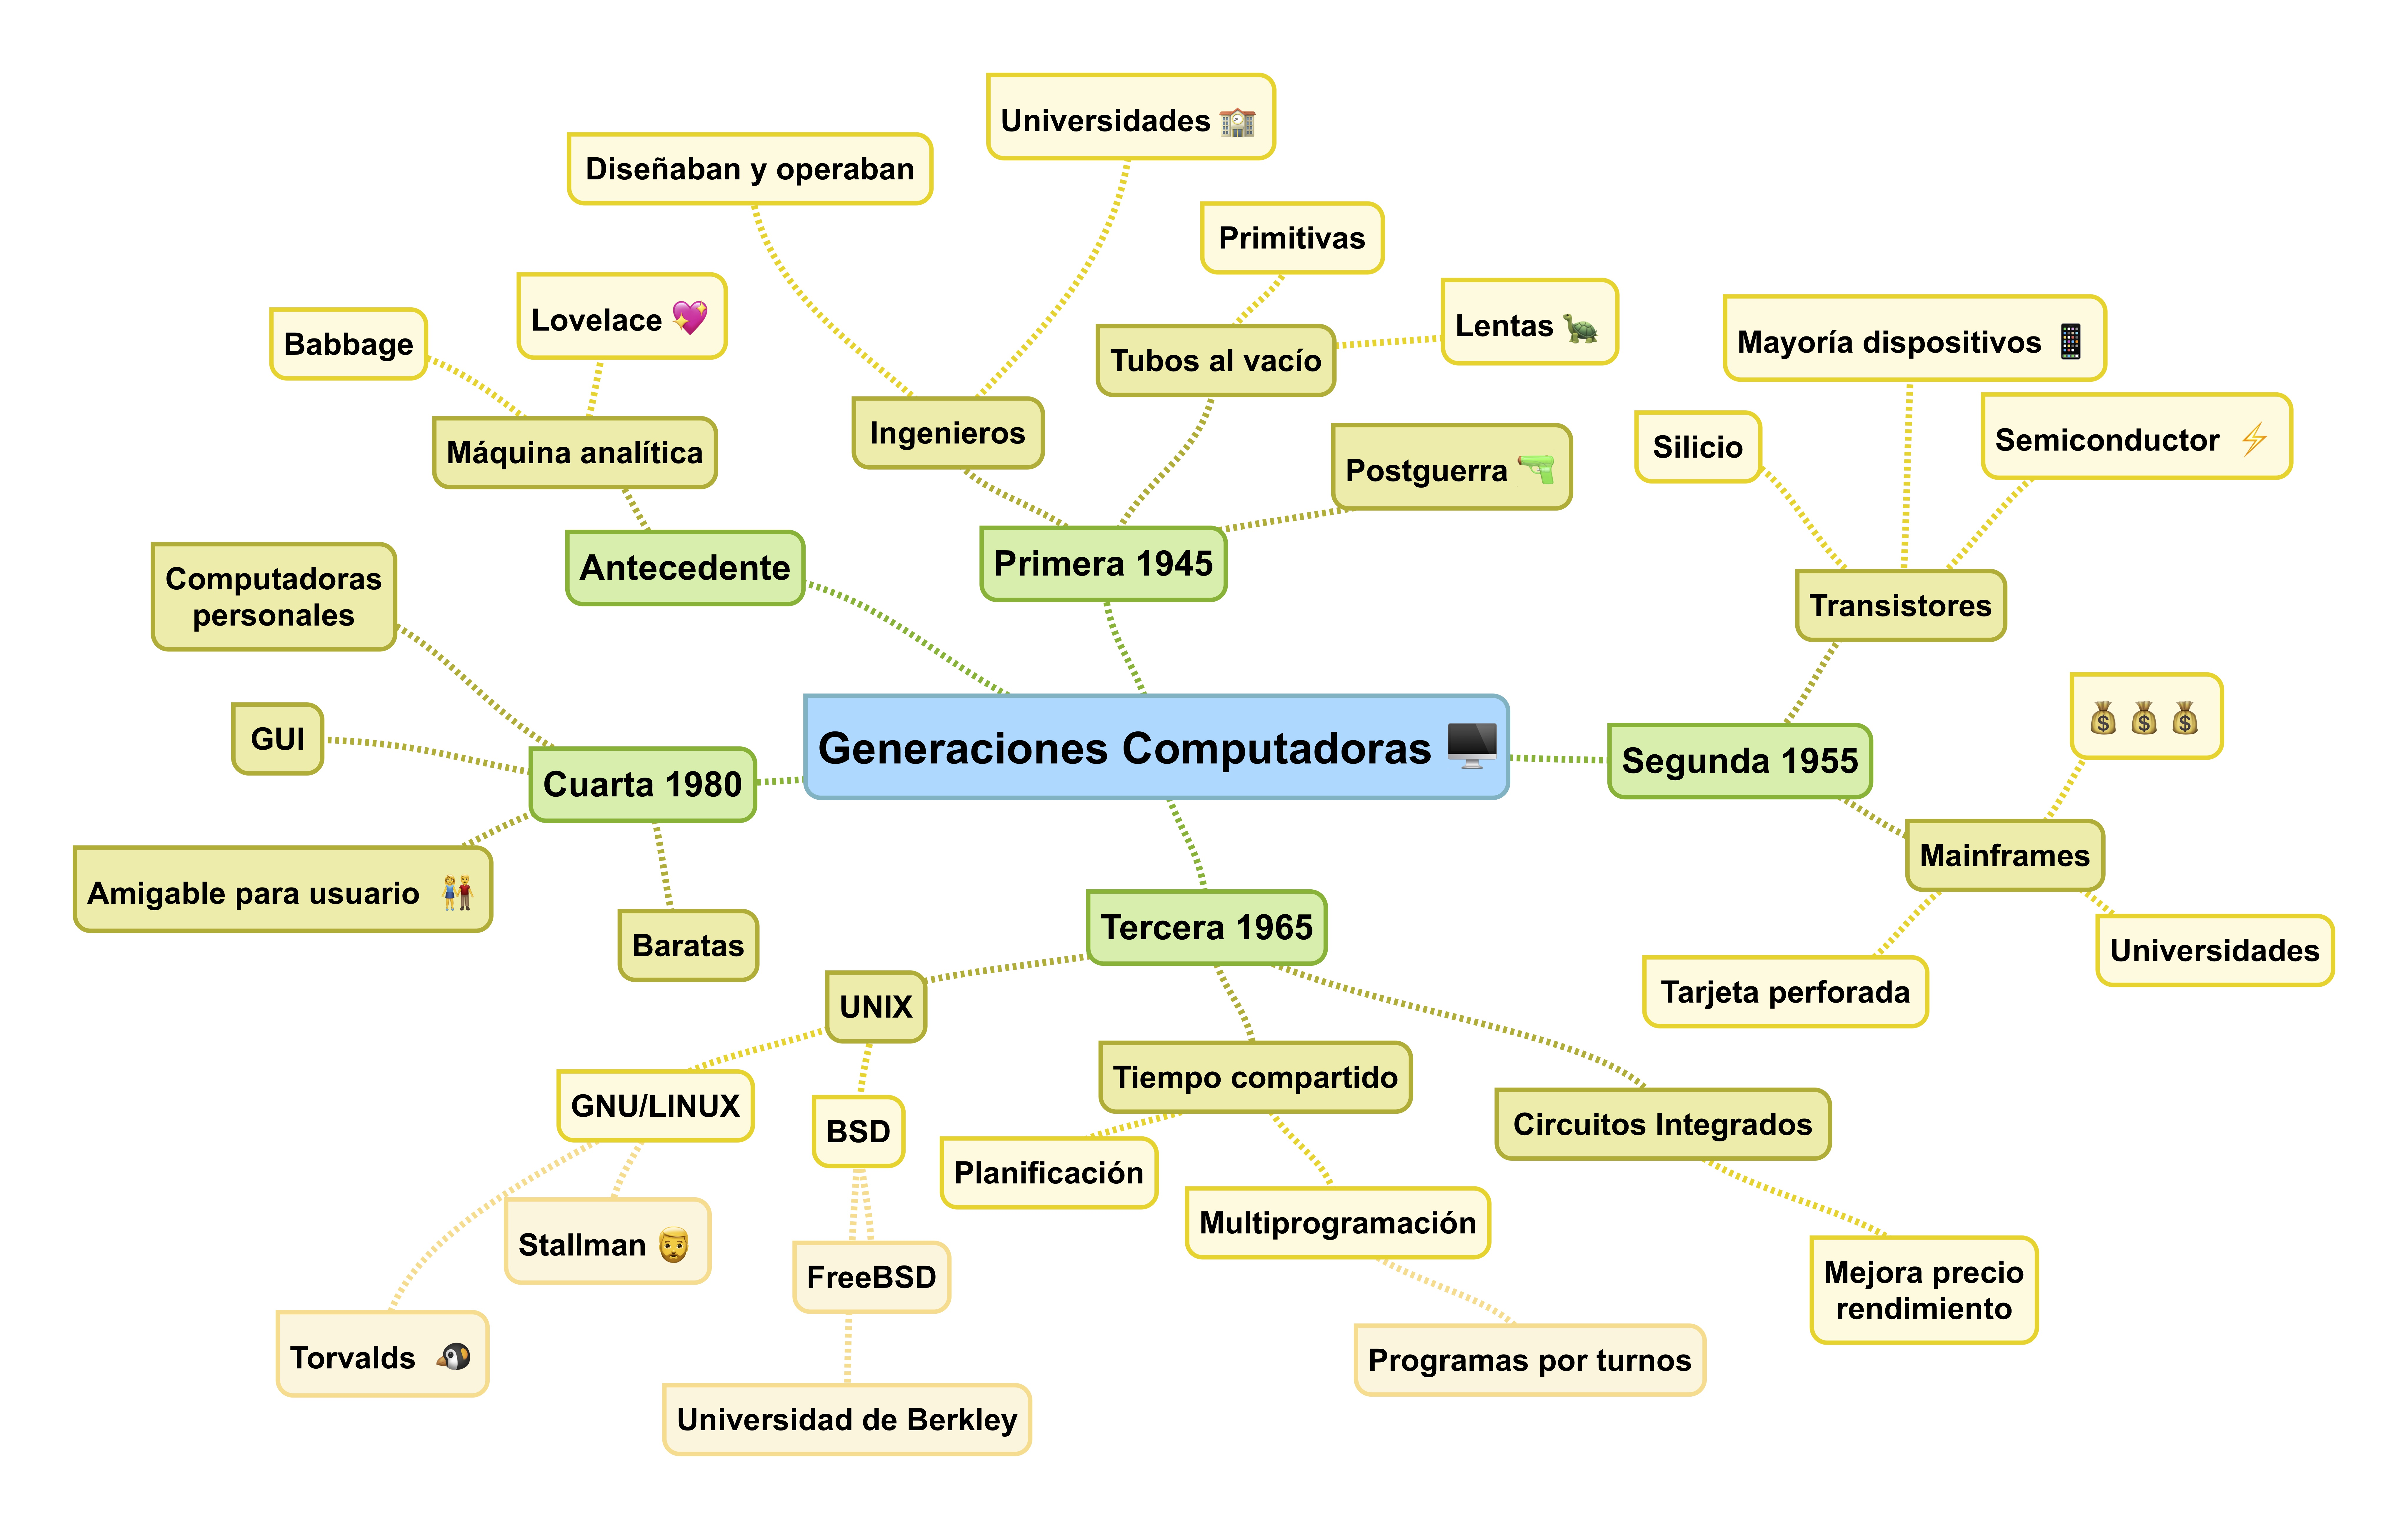
\includegraphics[scale=.05]{uno}
\caption{Mapa Generaciones de computadoras.}
\end{figure}
\justify 
Los antecedentes a las computadoras tienen su origen en la máquina de Babbage, creada por el matemático Charles Babbage, la cuál era programada por Ada Lovelace. Posteriormente se pueden definir la historia de las computadoras en 4 generaciones.
\begin{itemize}
\item Primera 1945. Utilizaban tubos al vacío, eran primitivas y lentas, creadas en la época post-guerra y los ingenieros eran los únicos con acceso a ellas.
\item Segunda 1955. El transistor revoluciono la industria de los dispositivos electrónicos, incluyendo las computadoras. Eran muy caras pero ahora además del gobierno las instituciones educativas tenían acceso a ellas y se programaban mediante tarjetas perforadas.
\item Tercera 1965. Los circuitos integrados permitieron una mejora en el precio y el rendimiento. Estas permitían a varios programas ejecutarse por turnos. Lo anterior en conjunto con la planificación hacóian posible el tiempo compartido para dotar a cada usuario de una parte de la computadora. Se da la creación de UNIX por Ritchie, se derivan varios sistemas operativos, entre ellos BSD desarrollado en la universidad de Berkley, y GNU/Linux que utilizaba el kernel hecho por Linus Torvals.
\item Cuarta 1980. Nació la era de la computadora personal el chip microprocesador. Se logró que un individuo tuviera su propia computadora personal, las cuales eran más abigables con un usuario promedio, en parte gracias a la creación de la Interfaz Gráfica de Usuario.
\end{itemize}

\end{document}